%!TEX root = ../main/main.tex

The Strahler number is similar to a centrality measure, in that it assigns a score to a node based on certain conditions. We can define the centrality measure using Strahler number in a sense that a higher Strahler number means higher centrality. It is important to remember that if a centrality measure admits a potential function, it will roots trees if, and only if, the potential function is symmetric (not necessarily works backwards). 

To determine if this centrality measure roots trees, we can define a potential function using the Strahler number. The potential function for a vertex v in a tree T is as follows:
    \begin{equation*}
        f_{S_{N}} (v,T) = \left\{ \begin{array}{llc}
             1 &   \text{if $v$ is a leaf of $T$ (i.e., $v$ does not have children)}  & \smallskip \\ 
              i & \text{if $v$ has one child $u$ with $f_{S_{N}}(u, T) = i$, and} \\
              	& \text{all other children have  $f_{S_{N}} < i$} \smallskip \\
              i + 1 &  \text{if $v$ has two or more children $u$ with $f_{S_{N}}(u, T) = i$} \\
              & \text{and no other children with $f_{S_{N}} > i$.} \\
             \end{array}
   \right.
    \end{equation*}
    
We can see that this potential function makes sense because the potential of a node it depends of their children (by definition of Strahler number).

We can see now if this function is symmetric knowing that the concept of the Strahler number, is to represent a directed graph and measure the centrality to different contexts. We can make a counter-example for this and observe that if we consider the graph:
\begin{center}
        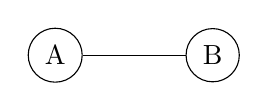
\begin{tikzpicture}
        \node[circle, draw] (A) at (0,0) {A};
        \node[circle, draw] (B) at (2,0) {B};
        \draw (A) -- (B);
    \end{tikzpicture}
\end{center}
In this example we can observe that, $f(A,T_{A,B}) =  f(B,T) = 0$ in such way that this is not symmetrical and in this sense does not root trees.

Knowing that this admits a potential function $f$ and $f$ is not symmetrical, by Theorem 11 in~\cite{RiverosSS23} it will not root trees. In other words, we cannot find the root of tree in all cases with this centrality. 

If this centrality does not roots trees we can explore other things like if this potential function in a monoids version, such this cannot happen because, this potential function implies a monoid that is not associative (which is not a monoid by definition), such leaf function can be drafted like:
\begin{equation}
    \max\{ x,y \}= \left\{ \begin{array}{lcc}
              \max\{x,y \} &   if  & x \neq y \\
             \\ \max\{ x,y \} + 1 & if  & x = y 
             \end{array}
   \right.
\end{equation}
This function can represent correctly the centrality of a single vertex , but, it can not represent a potential function (recursively) because is not associative (and thus is not a monoid). For example,
\begin{equation}
    \max\{ 1,\max\{ 1,2 \} \} = 2 \\
    \vspace{0.5cm}
    \max\{ \max\{ 1,1 \},2 \}  = 3 \\
    \vspace{0.5cm}
    \rightarrow 2 \neq 3
\end{equation}


